\chapter{Results}
\section{Overview}
Tests were conducted over a two week period between 31/03/25 and 13/04/25. Seven days worth of tests were exported from both machines for comparison and analysis. The results are discussed below, with pertinent tables included in the Appendix section. In comparison, the OONI database that is publicly available was analysed for the dates 13/03/25 to 13/04/25. 

It is important to recognize that, particularly in the case of Israel, different individuals may experience censorship of the Internet to varying degrees. The research focuses on replicating the experience of the average Israeli living in Tel Aviv. Having previously discussed the Gaza Strip, it is clear that the user experience varies greatly between the two areas. Further research may look at comparing Internet censorship experienced internally in Israel, but that is outside the scope of this work.

In the following section, the relevant context regarding the network conditions while gathering ground truth will be discussed. Having previously highlighted the varying levels at which internet censorship can be conducted, let us now define the specific network characteristics under which the OONI probe was run for both countries.

\subsection{Network Environment Context: Ireland}
As mentioned, the OONI CLI probe is running on a Raspberry Pi 5 connected to a home residential network over WiFi. The provider is Virgin Media (AS12388), registered under Liberty Global B.V. ISP (AS6830). 

Details regarding the operating system flashed to the Raspberry Pi and packages required for this are illustrated below in the 'Guide to Replicating Results.' 

\subsection{Network Environment Context: Israel}
Ground truth gathering in Israel was done using a virtual machine as described in the section on methodology. The virtual machine is operates within a data center hosted by O.M.C. COMPUTERS \& COMMUNICATIONS LTD (AS44709), downstream of its owner Kamatera Inc. (AS36007). This differs from the residential network that is being tested in Ireland.


\section{Website Connectivity Tests}


\subsection{Ground Truth via SSH}
\subsection{Native Website Connectivity Tests}
This section details the results of the daily web connectivity tests performed using the command \textit{ooniprobe run}. 

\begin{table}[H]
\centering
\caption{Summary of Tested vs. Blocked Websites by Country (Native to OONI)}
\begin{tabular}{lcc}
\toprule
\textbf{Country} & \textbf{Tested} & \textbf{Blocked} \\
\midrule
Ireland & 1695 & 25 \\
Israel    & 1695 & 16 \\   
\bottomrule
\end{tabular}
\label{tab:blocked_summary}
\end{table}




\subsection{my-websites.txt}
This file contains the additional 170 website connectivity tests I wished to conduct. The list was compiled with Griff Steinman, and additional tests relating to Israel were added. The contents can be found within the Appendix section. Below is a summary of the results from the daily running of this additional web connectivity test suite.

\begin{table}[H]
\centering
\caption{Summary of Blocked vs. Unblocked Websites by Country (my-websites)}
\begin{tabular}{lcc}
\toprule
\textbf{Country} & \textbf{Unblocked} & \textbf{Blocked} \\
\midrule
Ireland & 151 & 19 \\
Israel    & 155 & 15 \\   
\bottomrule
\end{tabular}
\label{tab:blocked_summary}
\end{table}

The following figure illustrates the blocking methods for the additional web connectivity tests. See Appendix section for a more detailed breakdown of positive results for each locale.

\begin{table}[H]
\centering
\caption{Distribution of Blocking Methods Detected in Ireland \&Israel}
\begin{tabular}{lcc}
\toprule
\textbf{Blocking Method} & \textbf{Ireland} & \textbf{Israel} \\
\midrule
TCP/IP         & 15 & 13 \\
DNS            & 1  & 1  \\
HTTP           & 1  & 1  \\
Error/Failure  & 3  & 0  \\
\bottomrule
\end{tabular}
\label{tab:blocking_methods_comparison}
\end{table}

\begin{table}[H]
\centering
\caption{Blocked Websites by Category and Country}
\begin{tabular}{lccc}
\toprule
\textbf{Category} & \textbf{Total Websites Tested} & \textbf{Ireland} & \textbf{Israel} \\
\midrule
Uncategorized                      & 34 & 4 & 4 \\
Piracy / Streaming / File Sharing  & 21 & 6 & 4 \\
News / Media                       & 34 & 1 & 0 \\
Adult Content                      & 21 & 0 & 0 \\
Creative / Educational / Misc      & 15 & 1 & 1 \\
General / National Services        & 19 & 1 & 1 \\
Streaming / Social Media           & 9  & 0 & 0 \\
Religious                          & 5  & 2 & 2 \\
VoIP / Communication               & 4  & 1 & 0 \\
Gambling                           & 2  & 1 & 1 \\
Email/Privacy Tools                & 3  & 1 & 0 \\
Adult / Alcohol                    & 2  & 1 & 1 \\
LGBTQ+                             & 1  & 1 & 1 \\
AI / Technology                    & 1  & 0 & 0 \\
\bottomrule
\end{tabular}
\label{tab:category_block}
\end{table}

\subsection{Investigating Aljazeera.com}
Upon initial testing of Aljazeera blocking in Israel, it was surprising to see no evidence of blocking. To investigate further it was decided that the content of the site should be examined and a variety of URLs belonging to it should be tested. Particular attention was given to articles that were critical of Israel.

The file sample\_aljazeeraurls.txt contains 100 URLs for articles hosted on https://aljazeera.com. Below are some helpful commands used to obtain the sitemap and extract URLs for testing. Wget was used to examine the contents of the web page, and the following was observed.

Despite preconceived notions, Aljazeera and its articles were not found to be blocked on AS44709. Reasons for this will be explored in the coming chapter.

\begin{figure} [H]
    \centering
    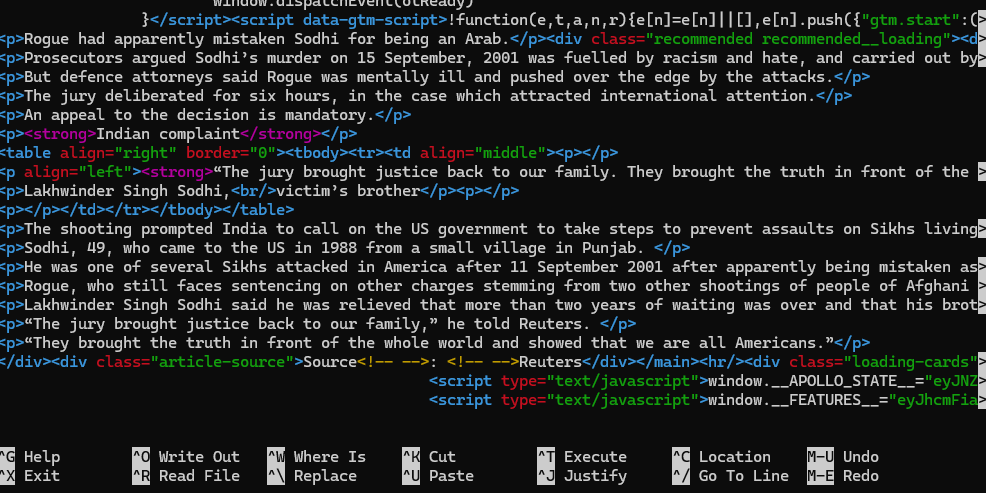
\includegraphics[width=1\linewidth]{wgetAljazeera.png}
    \caption{wget showing aljazeera.com content}
    \label{fig:enter-label}
\end{figure}


As seen above, I was able to see unblocked content from the site. Within Appendix, one can find a sample of articles being tested. 

\subsection{Public OONI Database}
In this section, the OONI database will be explored. As mentioned previously the period to be considered is 13/03/25 to 13/04/25. Below are screenshots of all web connectivity tests conducted in Ireland and Israel for these dates. 

\begin{figure} [H]
    \centering
    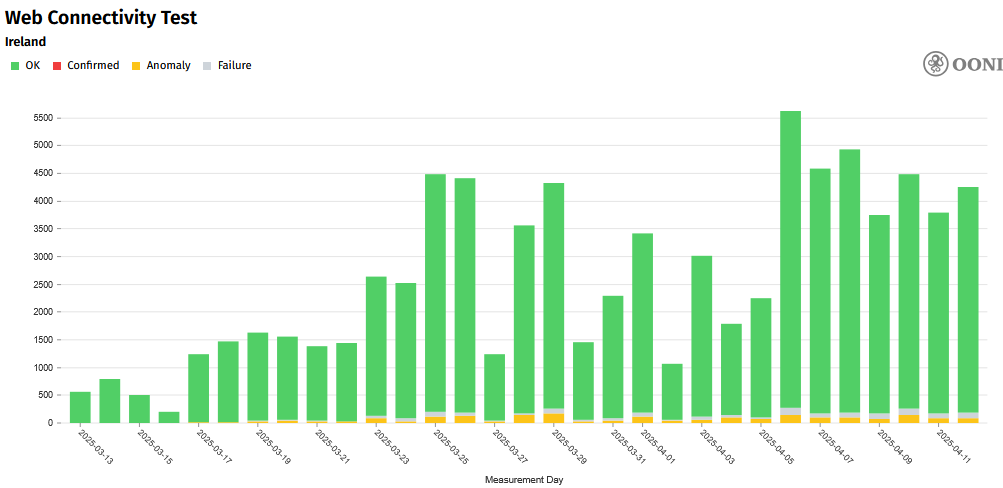
\includegraphics[width=1\linewidth]{IREWEBSOONIDB.png}
    \caption{Irish OONI Database Web connectivity tests 13/03-13/04}
    \label{fig:enter-label}
\end{figure}

\begin{figure} [H]
    \centering
    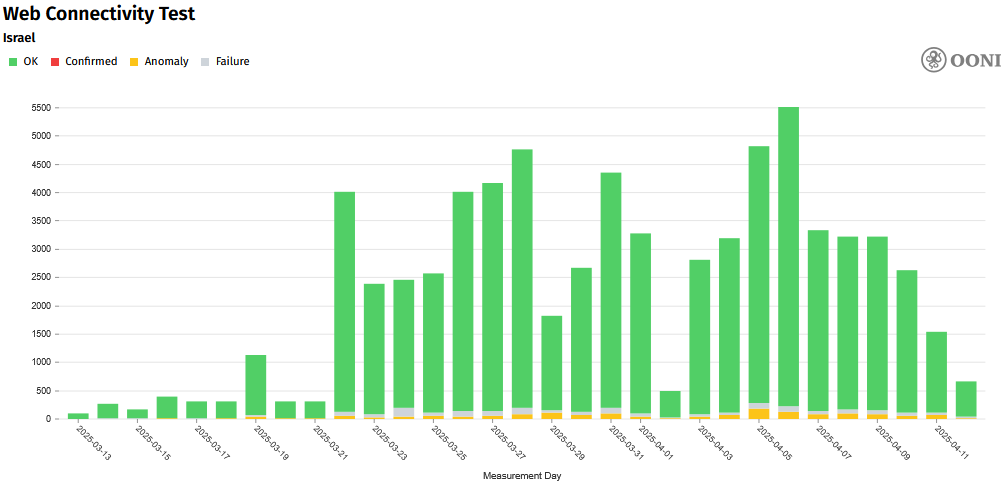
\includegraphics[width=1\linewidth]{ISRWEBSOONIDB.png}
    \caption{Israel OONI Database Web connectivity tests 13/03-13/04}
    \label{fig:enter-label}
\end{figure}

Further insight into this data can be seen through the proceeding table that documents a daily averages. 

\begin{table} [H]
\centering
\caption{Website Blocking based on Public OONI Data}
\begin{tabular}{lcc}
\toprule
\textbf{} & \textbf{Ireland} & \textbf{Israel} \\
% \midrule
Number of Websites Tested           & 2603 &  2299 \\
Number of Successful Connections    & 2491 & 2195 \\
Number of Anomalies                 & 67 & 53 \\
Number of Failures                  & 46 & 51 \\
\bottomrule
\end{tabular}
\label{tab:category_block}
\end{table}

By examining the publicly available data on Aljazeera and filtering based on ASN, an interesting picture emerges. There is clear evidence of large scale DNS tampering on certain ASNs, while others go unblocked. Prior to my testing using the VM in Tel Aviv, it was unknown whether O.M.C. COMPUTERS \& COMMUNICATIONS LTD (AS44709) was blocking this content. 

\begin{figure} [H]
    \centering
    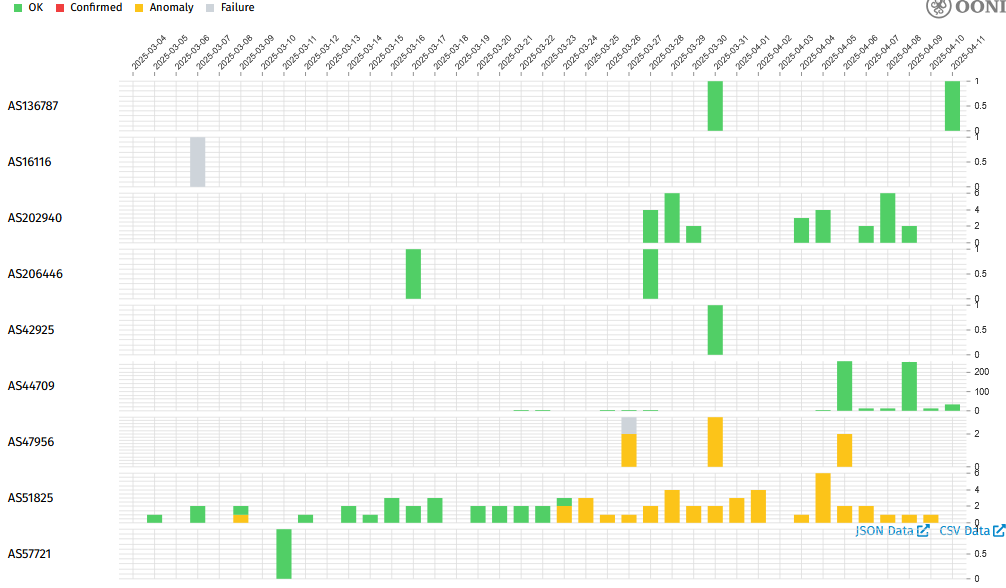
\includegraphics[width=1\linewidth]{ALJZRbyASN.png}
    \caption{OONI data (04/03/2025 - 11/04/2025) showing blocking of Alazeera.com grouped by ASN}
    \label{fig:enter-label}
\end{figure}



\section{Instant Messaging Tests}
By analysing the publicly available OONI data for both countries for the period of interest we can see little evidence of blocking of instant messaging platforms in either country.

\subsection{Public OONI Database: Ireland}
As seen in the below figures, there is little evidence to suggest network interference of instant messaging platforms in Ireland over the period considered.

\begin{figure} [H]
    \centering
    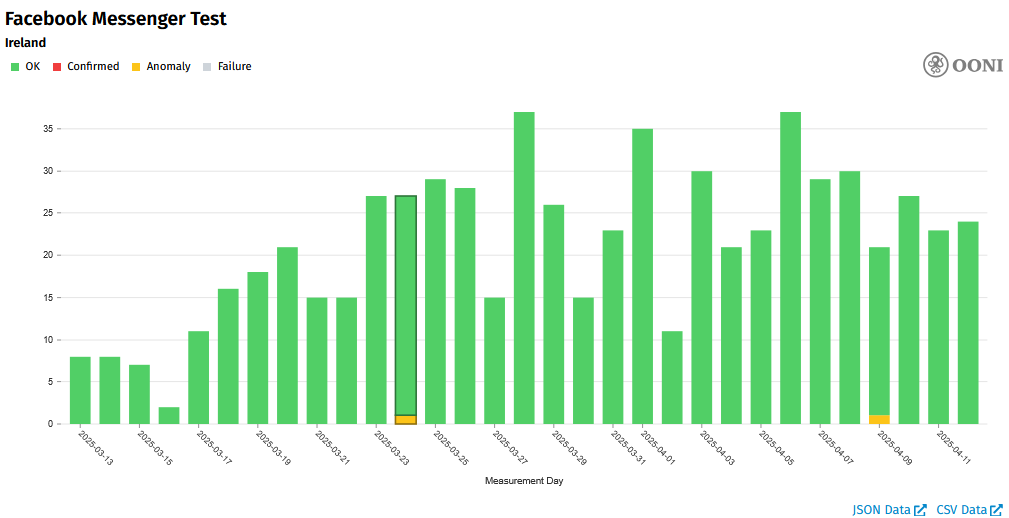
\includegraphics[width=0.5\linewidth]{IREOONIDBIMFB.png}
    \caption{Facebook Messenger test results for Ireland 13/03-13/04}
    \label{fig:enter-label}
\end{figure}

\begin{figure} [H]
    \centering
    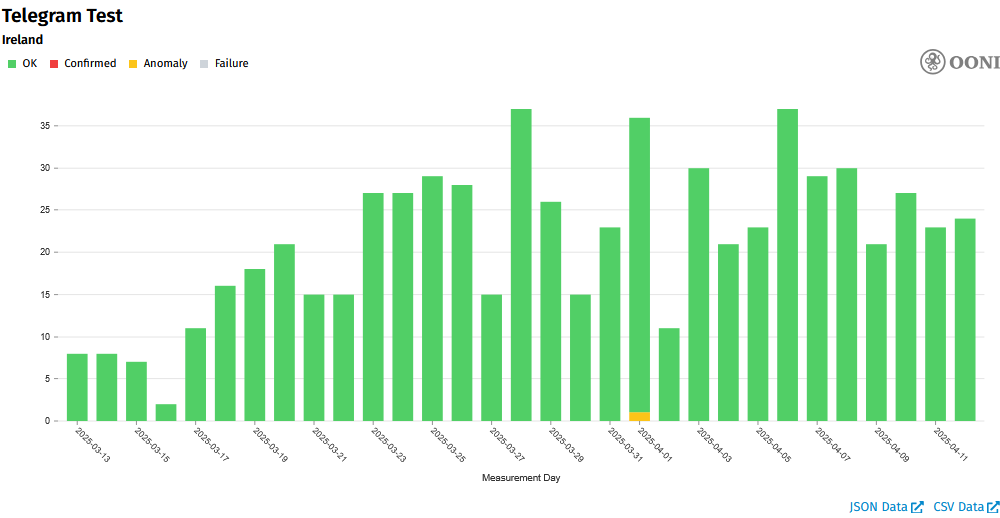
\includegraphics[width=0.5\linewidth]{IREOONIDBIMTL.png}
    \caption{Telegram test results for Ireland 13/03-13/04}
    \label{fig:enter-label}
\end{figure}

\begin{figure} [H]
    \centering
    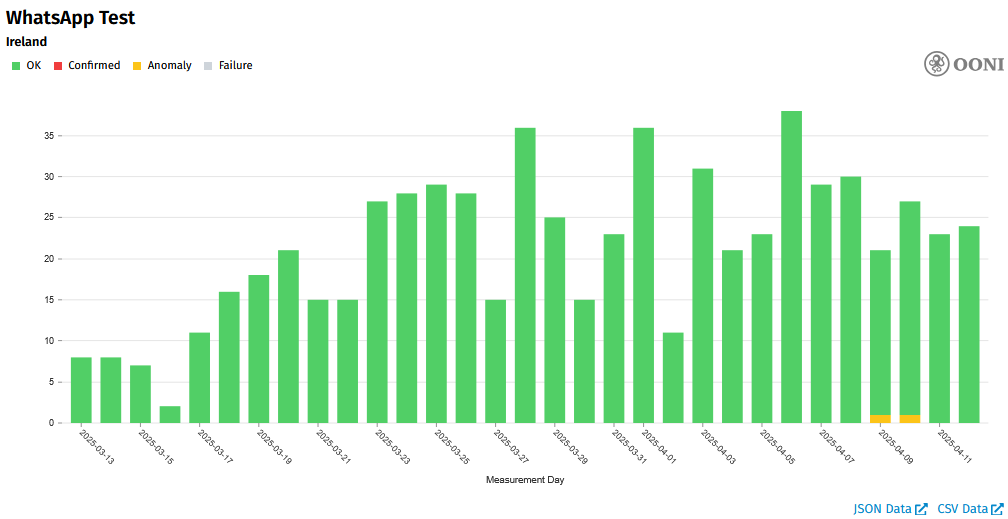
\includegraphics[width=0.5\linewidth]{IREOONIDBIMWHATS.png}
    \caption{WhatsApp test results for Ireland 13/03-13/04}
    \label{fig:enter-label}
\end{figure}

\begin{figure} [H]
    \centering
    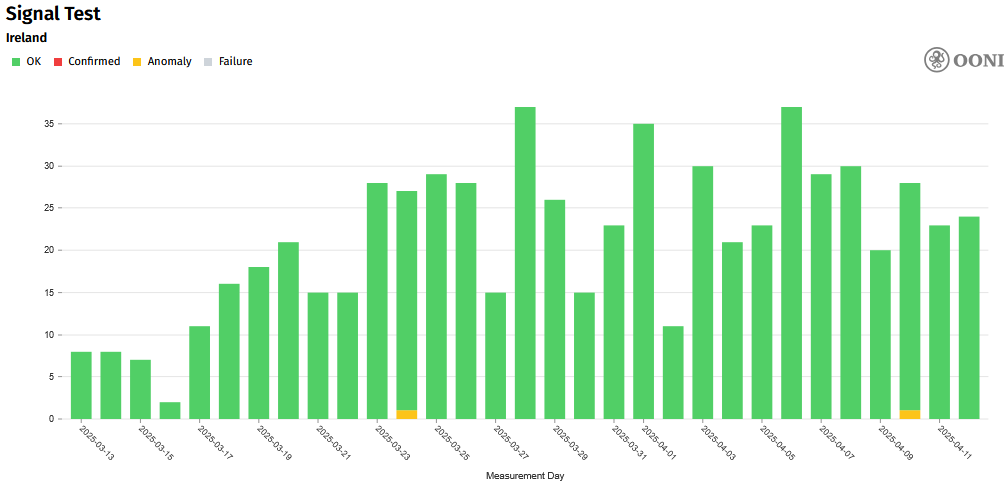
\includegraphics[width=0.5\linewidth]{IREOONIDBSIG.png}
    \caption{Signal test results for Ireland 13/03-13/04}
    \label{fig:enter-label}
\end{figure}



\subsection{Public OONI Database: Israel}
As seen in the below figures, there is little evidence to suggest network interference of instant messaging platforms in Israel over the period considered.

\begin{figure} [H]
    \centering
    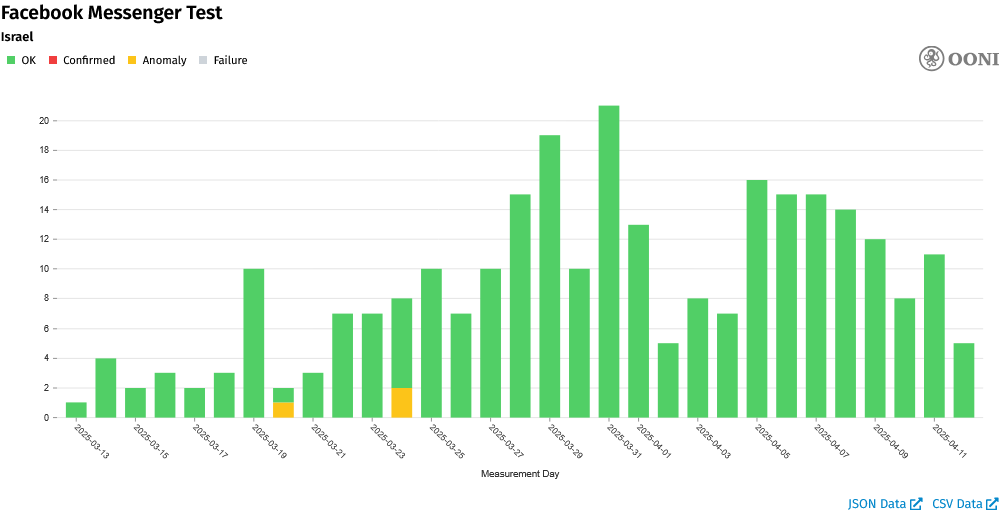
\includegraphics[width=0.5\linewidth]{ISROONIDBFB.png}
    \caption{Facebook Messenger test results for Israel 13/03-13/04}
    \label{fig:enter-label}
\end{figure}
\begin{figure} [H]
    \centering
    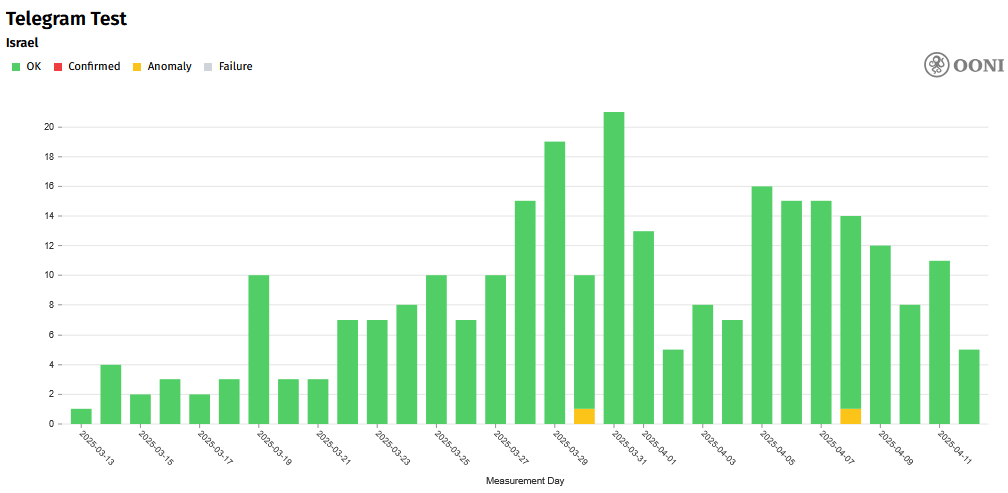
\includegraphics[width=0.5\linewidth]{ISROONIDBIM.png}
    \caption{Telegram test results for Israel 13/03-13/04}
    \label{fig:enter-label}
\end{figure}
\begin{figure} [H]
    \centering
    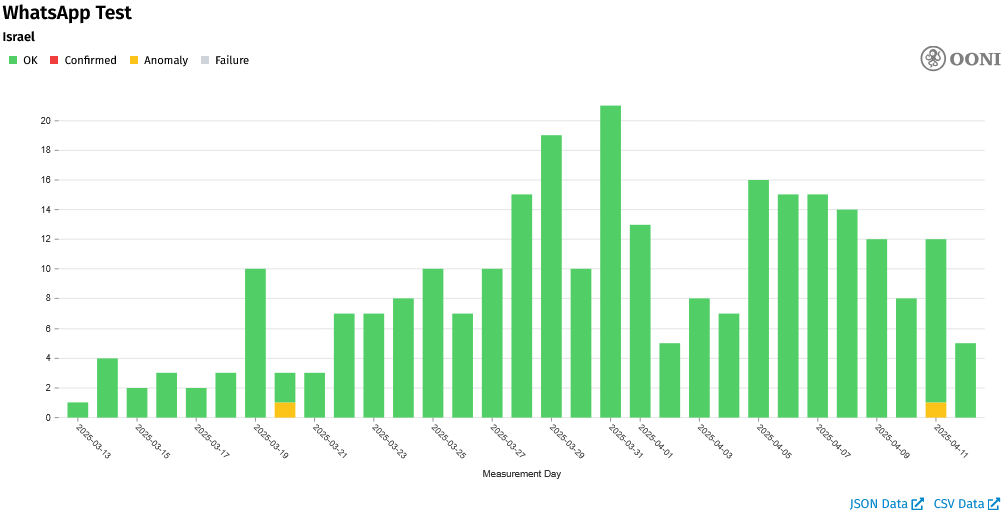
\includegraphics[width=0.5\linewidth]{ISROONIDBTEL.png}
    \caption{WhatsApp test results for Israel 13/03-13/04}
    \label{fig:enter-label}
\end{figure}
\begin{figure} [H]
    \centering
    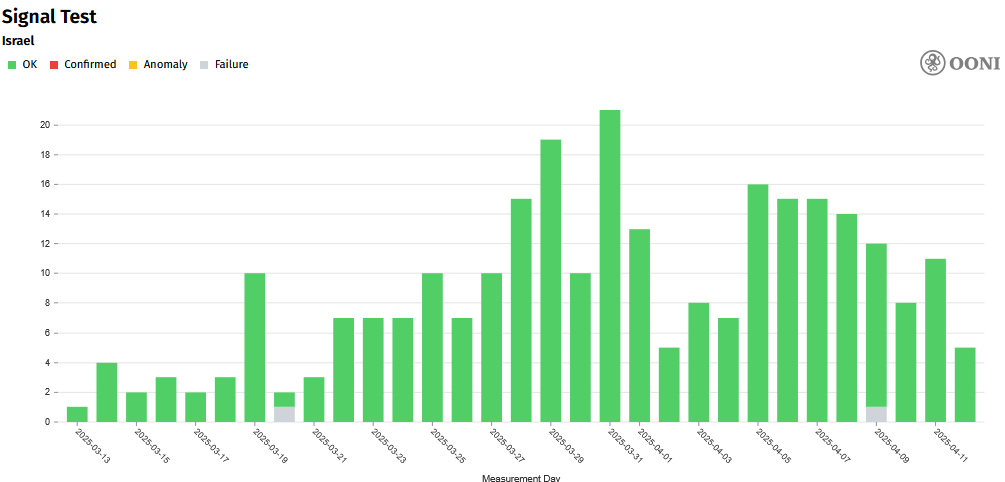
\includegraphics[width=0.5\linewidth]{ISROONIDBSIG.png}
    \caption{Signal test results for Israel 13/03-13/04}
    \label{fig:enter-label}
\end{figure}


\subsection{Ground Truth via SSH}
While running tests locally, no evidence for the blocking of instant messaging platforms was found in either Ireland or Israel. As seen in the above figures, there is little evidence in the OONI database to suggest either country interferes with instant messaging platforms. 


\section{Circumvention Tests}
\subsection{Public OONI Database: Ireland}

The majority of circumvention tests go unblocked in Ireland, however, certain ASNs show evidence of blocking. This can be see below.

\textbf{Ireland Circumvention Test Anomalies}
Based on data seen in the OONI database, TOR is not blocked by the majority of ASNs in Ireland. However, consistent blocking is seen in some networks. Over the period considered, there were seven instances of TOR being blocked, all attributed to HEAnet (AS 1213).

Psiphon appears to be blocked somewhat consistently on certain ASNs. The results are seen tabulated below, with a focus on ASNs containing anomalies.

\begin{table}[H]
\centering
\caption{Psiphon Circumvention Anomalies in Ireland}
\begin{tabular}{lccc}
\toprule
\textbf{Metric / ASN} & \textbf{Blocked} & \textbf{OK} & \textbf{\% Blocked} \\
\midrule
\textbf{Total}     & 82  & 575 & 12.48\% \\
\midrule
ASN 1213           & 57  & 6   & 90.48\% \\
ASN 6830           & 18  & 271 & 6.23\% \\
ASN 13280          & 5   & 13  & 27.78\% \\
ASN 9009           & 1   & 6   & 14.29\% \\
ASN 212238         & 1   & 0   & 100.00\% \\
ASN 8075           & 1   & 0   & 100.00\% \\
ASN 15751          & 1   & 8   & 11.11\% \\
\bottomrule
\end{tabular}
\label{tab:psiphon_ireland}
\end{table}



\begin{figure} [H]
    \centering
    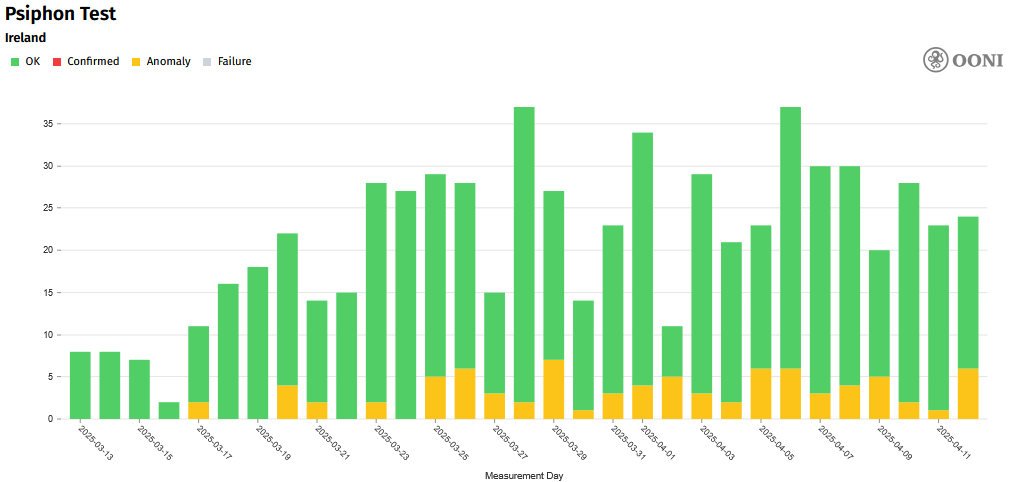
\includegraphics[width=0.5\linewidth]{IREDBPSI.png}
    \caption{Psiphon test results for Ireland 13/03-13/04}
    \label{fig:enter-label}
\end{figure}

\begin{figure} [H]
    \centering
    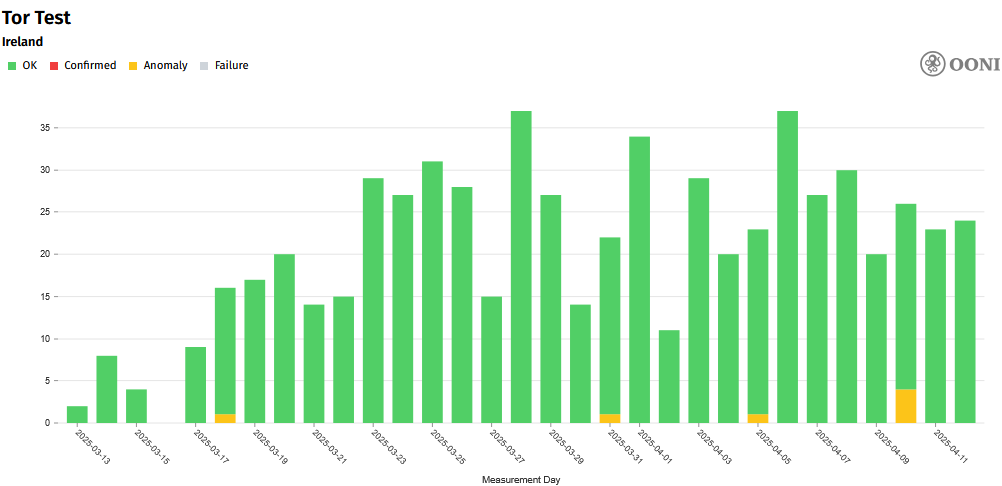
\includegraphics[width=0.5\linewidth]{IREDBTOR.png}
    \caption{TOR test results for Ireland 13/03-13/04}
    \label{fig:enter-label}
\end{figure}

\subsection{Public OONI Database: Israel}

Based on observations of the OONI database over the period of interest, TOR and Psiphon tests are not blocked in Israel. The only evidence of blocking comes from one autonomous system as described below.

\textbf{Israel Circumvention Test Anomalies}
ITC NG ltd (AS 202940) was responsible for 25 instances of blocking TOR connections and one instance of blocking Psiphon connections over the dates examined. This was the only ASN repsponsible for positive results. These anomalies are tabulated below.

\begin{table}[H]
\centering
\caption{Circumvention Results in Israel (ASN 202940)}
\begin{tabular}{lccc}
\toprule
\textbf{Tool} & \textbf{Blocked (Anomaly)} & \textbf{OK} & \textbf{\% Blocked} \\
\midrule
Psiphon & 1  & 27 & 3.57\% \\
Tor     & 25 & 3  & 89.29\% \\
\bottomrule
\end{tabular}
\label{tab:circumvention_israel}
\end{table}


\begin{figure} [H]
    \centering
    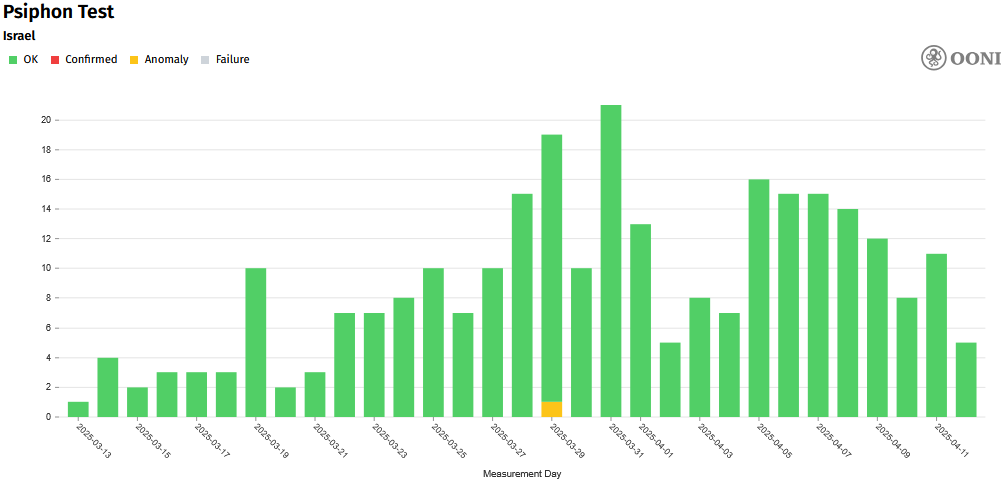
\includegraphics[width=0.5\linewidth]{ISROONIPSI.png}
    \caption{Psiphon test results for Israel 13/03-13/04}
    \label{fig:enter-label}
\end{figure}

\begin{figure} [H]
    \centering
    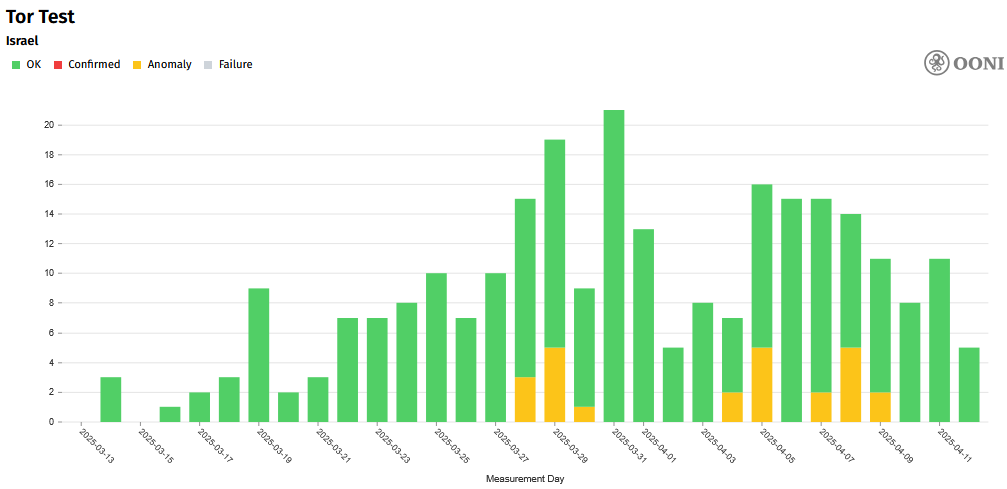
\includegraphics[width=0.5\linewidth]{ISROONITOR.png}
    \caption{TOR test results for Israel 13/03-13/04}
    \label{fig:enter-label}
\end{figure}

\subsection{Ground Truth via SSH}
No evidence for the blocking of TOR or Psiphon was found while running circumvention tests in either locale. This is consistent with the OONI database as in both countries, blocking appears inconsistent and AS specific.



\section{Middlebox Tests}
\subsection{Public OONI Database: Ireland}
In examining the OONI database for HTTP Invalid Request Line tests conducted in Ireland over the period of interest, only a handful of anomalies are observed. Out of the 660 HTTP Invalid Request Line tests conducted there were 5 anomalies. These instances belonged to M247 Europe SRL (AS9009), Vodafone Ireland Limited (AS15502) and Meteor Mobile Communications Limited (AS15751). A breakdown of the anomalies is seen below.

\begin{table}[H]
\centering
\caption{HTTP Invalid Request Line Test Anomalies in Ireland}
\begin{tabular}{lcc}
\toprule
\textbf{ASN} & \textbf{Anomalies} & \textbf{OK} \\
\midrule
\textbf{Total}   & 5 & 660 \\
\midrule
AS9009           & 3 & 4 \\
AS15502          & 1 & 103 \\
AS15751          & 1 & 9 \\
\bottomrule
\end{tabular}
\label{tab:http_invalid_ireland}
\end{table}



\begin{figure} [H]
    \centering
    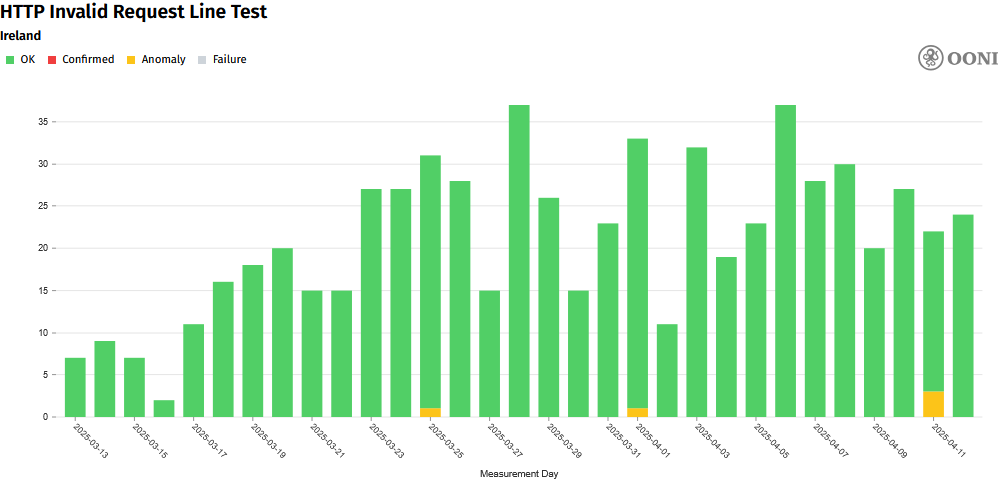
\includegraphics[width=0.5\linewidth]{IREOONIDBMB1.png}
    \caption{HTTP Invalid Request test results for Ireland 13/03-13/04}
    \label{fig:enter-label}
\end{figure}

Irish tests for HTTP Heaer Field Manipulation were less intriguing with only 6 anomalies over the period of interest. These were attributed to M247 Europe SRL (AS9009) and HEAnet (AS 1213) respectively. A breakdown of these results is seen below.


\begin{table}[H]
\centering
\caption{HTTP Header Field Manipulation Anomalies in Ireland}
\begin{tabular}{lccc}
\toprule
\textbf{ASN} & \textbf{Anomalies} & \textbf{OK} & \textbf{Percentage Anomalous} \\
\midrule
\textbf{Total}   & 6 & 648 & 0.91\% \\
\midrule
AS9009           & 2 & 1   & 66.67\% \\
AS1213           & 4 & 7   & 36.36\% \\
\bottomrule
\end{tabular}
\label{tab:http_header_ireland}
\end{table}

\begin{figure} [H]
    \centering
    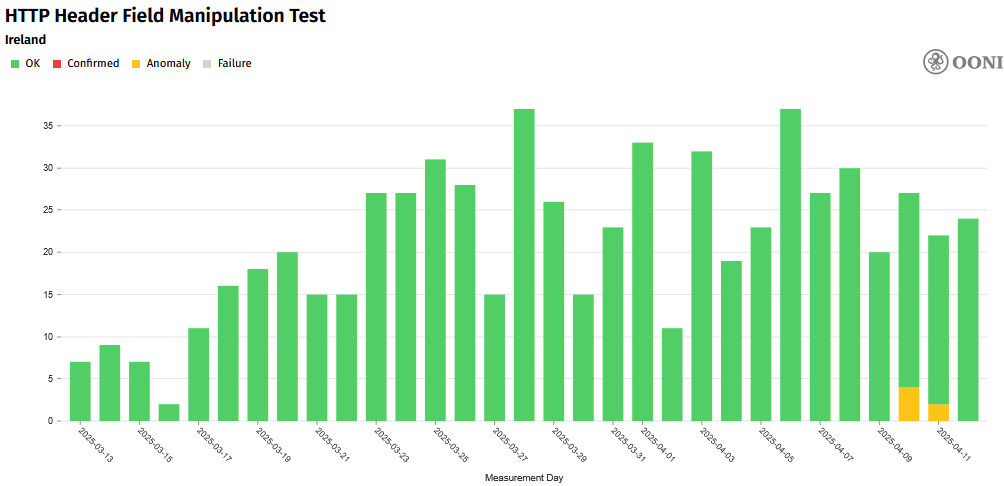
\includegraphics[width=0.5\linewidth]{IREOONIDBMB2.png}
    \caption{HTTP Header Field Manipulation test results for Ireland 13/03-13/04}
    \label{fig:enter-label}
\end{figure}







\subsection{Public OONI Database: Israel}
Only one instance of HTTP a Invalid Request Line anomaly was seen in Israel over the period of interest and belonged to XFone 018 Ltd (AS47956). 


\begin{figure} [H]
    \centering
    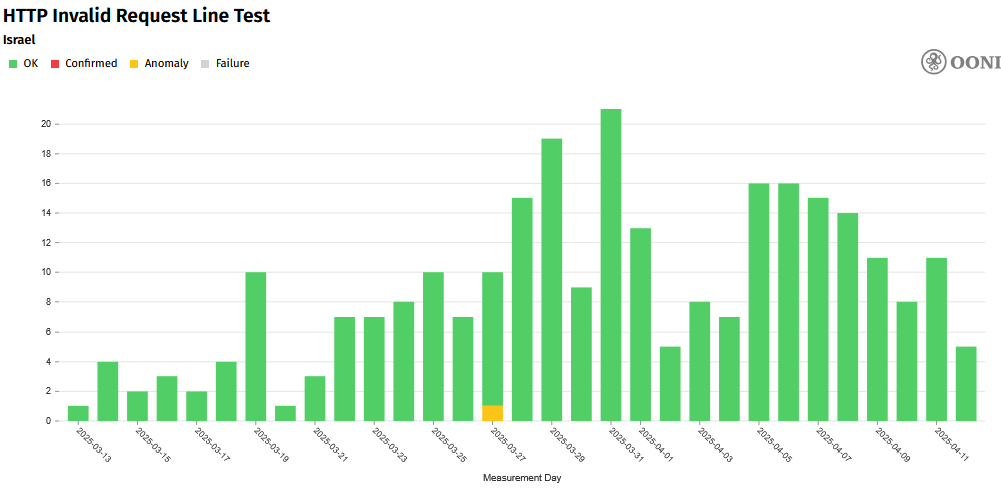
\includegraphics[width=0.5\linewidth]{ISROONIDBMB1.png}
    \caption{HTTP Invalid Request test results for Israel 13/03-13/04}
    \label{fig:enter-label}
\end{figure}

On the other hand, HTTP Header Field Manipulation test results for Israel were quite interesting. Anomalies were attributed to three different ASNs: Cellcom Fixed Line Communication L.P (AS1680), ITC NG ltd (AS202940) and XFone 018 Ltd (AS47956). The breakdown of these results is tabulated below.

\begin{table}[H]
\centering
\caption{HTTP Header Field Manipulation Anomalies in Israel}
\begin{tabular}{lccc}
\toprule
\textbf{ASN} & \textbf{Anomalies} & \textbf{OK} & \textbf{Percentage Anomalous} \\
\midrule
\textbf{Total}       & 35 & 237 & 12.87\% \\
\midrule
AS202940             & 25 & 4   & 86.21\% \\
AS1680               & 9  & 3   & 75.00\% \\
AS47956              & 1  & 7   & 12.50\% \\
\bottomrule
\end{tabular}
\label{tab:http_header_israel}
\end{table}


\begin{figure} [H]
    \centering
    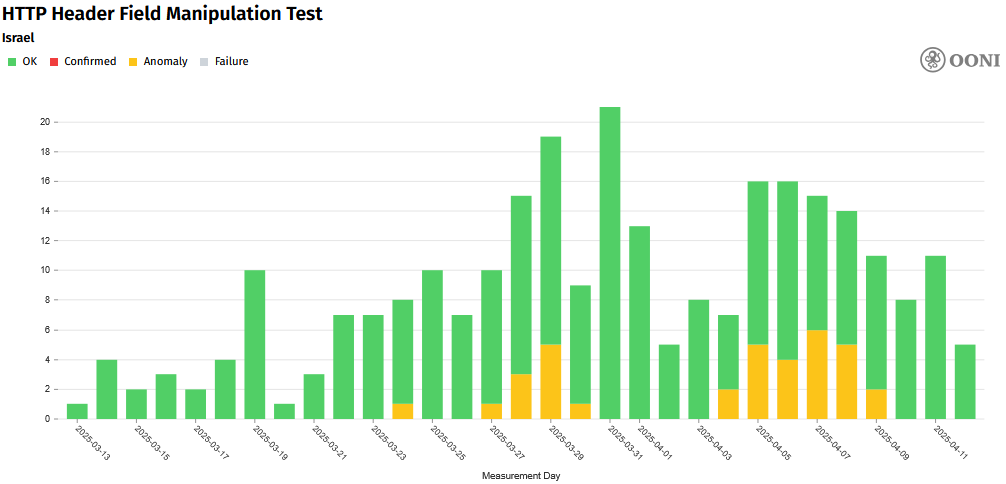
\includegraphics[width=0.5\linewidth]{ISROONIDBMB2.png}
    \caption{HTTP Header Field Manipulation test results for Israel 13/03-13/04}
    \label{fig:enter-label}
\end{figure}

\subsection{Ground Truth via SSH}
Results of running middlebox tests locally in both countries were uninteresting and no evidence of their presense was noted. However, as seen above Cellcom Fixed Line Communication L.P (AS1680) and ITC NG ltd (AS202940) are responsible for a significant number of positive with a majority of measurements showing interference. 



\section{Comparitive Analysis: Ireland vs. Israel}
\subsection{Summary: Irish Internet Censorship}
\subsection{Summary: Israeli Internet Censorship}
\subsection{}

\section{Guide to Replicating Results}

\subsection{Investigating Aljazeera.com}
Below are some commands I found helpful while investigating aljazeera.com.

\begin{figure} [H]
    \centering
    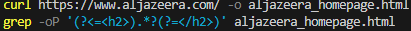
\includegraphics[width=1\linewidth]{AljazeeraURLs1.png}
    \caption{Using curl and grep to scrape URLs for articles}
    \label{fig:enter-label}
\end{figure}

\begin{figure} [H]
    \centering
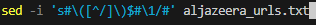
\includegraphics[width=1\linewidth]{AljazeeraComs2.png}
    \caption{Inserting a dash after each URL, can now be ran with OONI}
    \label{fig:enter-label}
\end{figure}


\subsection{Raspberry Pi Setup}
\textbf{Operating System}
The operating system used was the latest available version of Raspberry Pi OS (64-bit) at the time of testing. It was flashed using the Raspberry Pi Imager application over USB. 

\begin{flushleft}
\hspace{1em}\textbf{Raspberry Pi OS (64-bit)}\\[0.5em]
\hspace{1em}Release date: November 19th 2024\\[0.5em]
\hspace{1em}System: 64-bit\\[0.5em]
\hspace{1em}Kernel version: 6.6\\[0.5em]
\hspace{1em}Debian version: 12 (bookworm)
\end{flushleft}


\textbf{Packages Installed}
In order to install the OONI probe CLI, the guide 'Install OONI Probe CLI on Debian/Ubuntu Linux' \cite{ooni-cli-install} was followed. The process was similar to that of installing on the Israeli VM. One obstacle faced in both instances were OpenPGP errors. To solve, the permissions for OONI probe had to be updated to bypass PGP signature verification. To do this, /etc/apt/sources.list.d/ooniprobe.list was edited to include '[trusted=yes]'

\begin{figure} [H]
    \centering
    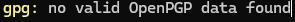
\includegraphics[width=0.75\linewidth]{PGPERROR.png}
    \caption{PGP Error installing CLI}
    \label{fig:enter-label}
\end{figure}


